% !TEX TS-program = lualatex

% Основано на  презентациях Юрия Викторовича Литвинова:
% https://github.com/yurii-litvinov/courses/tree/master/programming-1st-semester/02-intro
% https://github.com/yurii-litvinov/courses/tree/master/programming-1st-semester/04-complexity
% https://github.com/yurii-litvinov/courses/tree/master/programming-1st-semester/06-sortings
% https://github.com/yurii-litvinov/courses/tree/master/programming-1st-semester/09-structs-modules-files
% https://github.com/yurii-litvinov/courses/tree/master/programming-1st-semester/11-dynamic-structures
\documentclass[aspectratio=169]{beamer}

%%% Setup fonts.
\usepackage{fontspec}
%% Fancy fonts
\setmainfont{Iosevka Etoile}
\setsansfont{Iosevka Aile}
\setmonofont{Iosevka}

%% Default fonts
% \setmainfont{CMU Serif}
% \setsansfont{CMU Sans Serif}
% \setmonofont{CMU Typewriter Text}

%% Math
\usepackage{amsmath, amsfonts, amsthm, mathtools} % Advanced math tools.
\usepackage{amssymb}

\usepackage{unicode-math} % Allow TTF and OTF fonts in math and allow direct typing unicode math characters.
\unimathsetup{
    warnings-off={
            mathtools-colon,
            mathtools-overbracket
        }
}
% \setmathfont{Lete Sans Math}[CharacterVariant={3,6},StylisticSet={4}]
\setmathfont{Latin Modern Math}

%%% Language settings.
\usepackage{polyglossia}
\setdefaultlanguage{russian}
\setotherlanguage{english}

%%% Beamer settings
% Themes
\usetheme{Boadilla}
\useinnertheme{circles}
\usecolortheme[style=Latte, accent=Blue]{catppuccin}
% Templates
\setbeamertemplate{navigation symbols}{} %remove navigation symbols
\setbeamertemplate{page number in head/foot}[appendixframenumber]
\setbeamertemplate{title page}[default][colsep=-4bp,rounded=true]

%%% Colors
\hypersetup{colorlinks}
\usepackage{catppuccinpalette}

\usepackage{booktabs}

\usepackage{minted}
\usemintedstyle{catppuccin-latte}

\usepackage{csquotes}

% \usepackage{xurl}

%% Custom commands
\NewDocumentCommand{\attribution}{mmmmm}{\href{#1}{#2}, \href{#3}{#4}, #5}
\NewDocumentCommand{\attributionCCThreeWikimedia}{mm}{\attribution{#1}{#2}{https://creativecommons.org/licenses/by-sa/3.0}{CC BY-SA 3.0}{via Wikimedia Commons}}
\NewDocumentCommand{\attributionPDWikimedia}{mm}{\attribution{#1}{#2}{}{Public Domain}{via Wikimedia Commons}}


\usepackage{xurl}

%%% Meta

\title{Стек и очередь}
\author{Николай Пономарев}
\date{2 октября 2025 г.}
\titlegraphic{
\includegraphics[height=1cm]{../фирменный блок_серый.pdf}}
\subject{Стек и очередь на указателях. Практика по написанию стека.}

\begin{document}

\begin{frame}[plain, noframenumbering]
    \titlepage
\end{frame}

\begin{frame}[fragile]
    \frametitle{Замечания по домашкам}

    \begin{itemize}
        \item Следуйте стилю кода!
        \item Не путайте соглашения в Python и в Си
        \item Инициализируйте переменные
        \item Стиль WebKit и настройки Clang Format расходятся :(
              \begin{itemize}
                  \item \mintinline{c}|int *a| vs. \mintinline{c}|int* a|
                  \item Выберите один и используйте его единообразно!
              \end{itemize}
        \item Дата в названии Pull Request~--- плохо
              \begin{itemize}
                  \item Лучше использовать номер задачки или её человеческое название
                  \item Можно даже так: \enquote{ДЗ № X.X Название задачки, Фамилия Имя}
              \end{itemize}
    \end{itemize}

\end{frame}

\begin{frame}[fragile]
    \frametitle{Рекомендации по домашкам}
    \begin{itemize}
        \item Нужен содержательный main и пример использования
        \item Старайтесь, чтобы весь ввод-вывод был в main-е
        \item Старайтесь писать переиспользуемый код (будто ваши функции кому-то могут понадобиться), проектируйте для переиспользования
              % \item В заголовочных файлах должны быть только объявления
        \item Не выкладывайте .exe, .o и т.п.
        \item Пожалуйста, не называйте массив \enquote{Arr}, стек \enquote{stek} и т.д.
        \item Закомментированный код не нужен
        \item \mintinline{c}|a == true| равносильно \mintinline{c}|a == true == true| и т.д., пишите if (a) или if~(!a)
        \item Именование файлов --- тоже в camelCase
              % \item Сброс входного потока: \mintinline{c}|scanf("%*[^\n]");| или \mintinline{c}|while (getchar() != '\n')|
    \end{itemize}
\end{frame}

\begin{frame}[fragile]
    \frametitle{Ещё рекомендации}
    \begin{itemize}
        \item Тернарный оператор: \mintinline{c}|printf(x == 0 ? "true" :  "false");|
              % \item Булевые функции возвращают true или false, не 0 или 1
        \item Используйте assert (из assert.h) для проверки инвариантов
        \item Не пишите \mintinline{c}|x += 1|, пишите \mintinline{c}|++x|
        \item Надо ли передавать в функции длину строки?
        \item Можно ли считать strlen в цикле?
        \item Не возвращайте 0, если программа завершилась с ошибкой
        \item Не используйте exit
              \begin{itemize}
                  \item Если функция может не выполниться, используйте коды возврата
              \end{itemize}
    \end{itemize}
\end{frame}

\begin{frame}
    \frametitle{Коды возврата}
    \begin{scriptsize}
        \inputminted[firstline=2, lastline=16]{c}{fib1.c}
        ...
        \inputminted[firstline=21, lastline=26]{c}{fib1.c}
    \end{scriptsize}
\end{frame}

\begin{frame}
    \frametitle{Или так}
    \begin{scriptsize}
        \inputminted[firstline=2, lastline=13]{c}{fib2.c}
        ...
        \inputminted[firstline=17, lastline=22]{c}{fib2.c}
    \end{scriptsize}
\end{frame}

\begin{frame}[fragile]
    \frametitle{if-else и return}
    \begin{minted}{c}
void f(int x) {
    if (x == 0) {
        ...
    } else {
        ...
    }
}
        \end{minted}
    или
    \begin{minted}{c}
void f(int x) {
    if (x == 0) {
        ...
        return;
    }
    ...
}
        \end{minted}
\end{frame}

\begin{frame}[fragile]
    \frametitle{Ещё комментарии}
    Не пишите так:
    \begin{minted}{c}
if (x == 10)
    return true;
else
    return false;
        \end{minted}
    Пишите так:
    \begin{minted}{c}
return x == 10;
        \end{minted}
\end{frame}

\begin{frame}[fragile]
    \frametitle{И ещё комментарии}
    \begin{itemize}
        \item Предупреждения компилятора
        \item Выделение памяти с инициализацией нулями
    \end{itemize}
    \begin{minted}{c}
int* array = (int*)calloc(size, sizeof(int));
if (array == NULL) {
    printf("Всё очень плохо :(")
    return 1;
}
...
free(array);
        \end{minted}
\end{frame}

\begin{frame}[fragile]
    \frametitle{Структуры I/II}
    \begin{itemize}
        \item Способ группировки родственных по смыслу значений
        \item Структура --- это тип
              \begin{itemize}
                  \item В памяти представляется как поля, лежащие друг за другом, возможно, с \enquote{дырками} (padding)
                  \item Объявляется вне функции
              \end{itemize}
    \end{itemize}
    \begin{columns}[t]
        \begin{column}{0.45\linewidth}
            Объявление структуры:
            \begin{minted}{c}
struct Point {
    int x;
    int y;
};
            \end{minted}
        \end{column}
        \begin{column}{0.45\linewidth}
            Использование:
            \begin{minted}{c}
struct Point p;
p.x = 10;
            \end{minted}
        \end{column}
    \end{columns}
\end{frame}

\begin{frame}[fragile]
    \frametitle{Структуры II/II}
    \begin{itemize}
        \item Или, чтобы \mintinline{c}{struct} каждый раз не писать:
              \begin{minted}{cpp}
typedef struct {
    int x;
    int y;
} Point;
            \end{minted}
              \begin{itemize}
                  \item \mintinline{c}{typedef} --- объявление синонима типа
              \end{itemize}
        \item Использование:
              \begin{minted}[extrakeywordstype={Point}]{c}
Point p = {10, 20};
printf("(%d, %d)", p.x, p.y);
            \end{minted}
        \item Продвинутая инициализация:
              \begin{minted}[extrakeywordstype={Point}]{c}
Point p = {.x = 10, .y = 20};
            \end{minted}
    \end{itemize}
\end{frame}

\begin{frame}
    \frametitle{Указатели и структуры}
    Структуры и указатели настолько часто используются вместе, что есть оператор \texttt{->} (разыменовать указатель на структуру и обратиться к её полю)
    \begin{footnotesize}
        \inputminted[extrakeywordstype={Point}, firstline=8, lastline=20]{c}{structPointer.c}
    \end{footnotesize}
    То же самое, что \mintinline{c}|(*p).x| и \mintinline{c}|(*p).y|
\end{frame}

\begin{frame}[fragile]
    \frametitle{Операция взятия адреса}
    \inputminted[extrakeywordstype={Point}, firstline=8, lastline=17]{c}{structRef.c}
\end{frame}

\begin{frame}[fragile]
    \frametitle{Структуры и строки}
    \begin{footnotesize}
        \inputminted[extrakeywordstype={PhoneBookEntry}, firstline=4, lastline=22]{c}{structStr.c}
    \end{footnotesize}
\end{frame}


\begin{frame}[fragile]
    \frametitle{Структуры могут указывать сами на себя}
    \begin{footnotesize}
        \inputminted[extrakeywordstype={ListElement}, firstline=4, lastline=22]{c}{structSelf.c}
    \end{footnotesize}
\end{frame}

\begin{frame}
    \frametitle{Стек на указателях}
    Структура данных, в которой элемент можно добавлять только в начало и забирать только из начала (LIFO, Last In --- First Out)
    \begin{columns}
        \begin{small}
            \begin{column}{0.55\textwidth}
                \begin{itemize}
                    \item Может хранить \enquote{сколько угодно} данных
                          \begin{itemize}
                              \begin{scriptsize}
                                  \item Можно сделать стек ещё на массивах, но тогда он будет ограничен по размеру
                              \end{scriptsize}
                          \end{itemize}
                \end{itemize}
            \end{column}
        \end{small}
        \begin{column}{0.45\textwidth}
            \begin{center}
                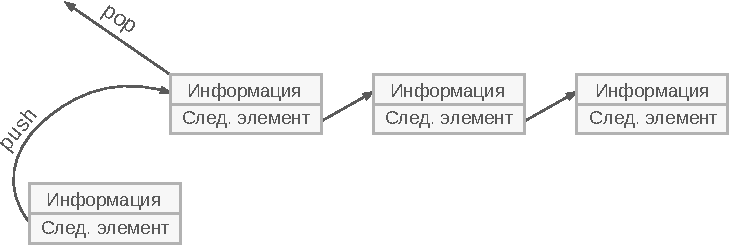
\includegraphics[width=0.95\textwidth]{stack.pdf}
                \begin{tiny}
                    \href{https://commons.wikimedia.org/wiki/File:Stack_preview.svg}{Vectorization:  Alhadis}, \href{https://creativecommons.org/licenses/by-sa/3.0}{CC BY-SA 3.0}, via Wikimedia Commons
                \end{tiny}
            \end{center}
        \end{column}
    \end{columns}
    \begin{itemize}
        \item Используется везде
              \begin{itemize}
                  \begin{scriptsize}
                      \item Для организации рекурсии
                      \item Для синтаксического анализа программ
                      \item Для проверки корректности скобок
                      \item Для арифметических вычислений
                      \item Для исполнения программ (.NET --- пример стековой машины)
                      \item ...
                  \end{scriptsize}
              \end{itemize}
    \end{itemize}
\end{frame}

\begin{frame}
    \frametitle{Очередь}
    Структура данных, в которой элемент можно добавлять только в конец и забирать только из начала (FIFO, First In --- First Out)
    \begin{columns}
        \begin{column}{0.6\textwidth}
            \begin{itemize}
                \item Используется для
                      \begin{itemize}
                          \item Обмена сообщениями между параллельными потоками
                          \item Обработки событий от пользователя или от операционной системы
                          \item ...
                      \end{itemize}
            \end{itemize}
        \end{column}
        \begin{column}{0.4\textwidth}
            \begin{center}
                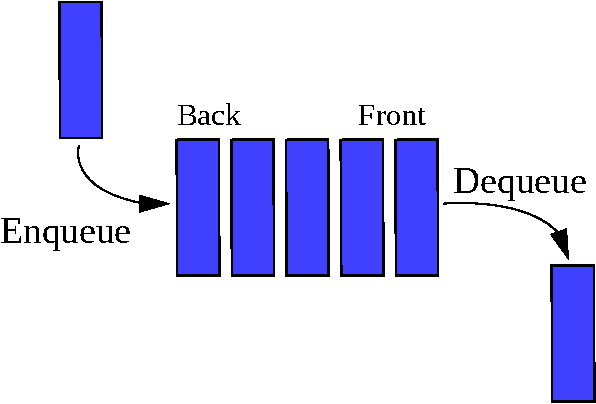
\includegraphics[width=0.9\textwidth]{queue.pdf}
                \begin{tiny}
                    \href{https://commons.wikimedia.org/wiki/File:Data_Queue.svg}{Vegpuff/Wikipedia}, \href{https://creativecommons.org/licenses/by-sa/3.0}{CC BY-SA 3.0}, via Wikimedia Commons
                \end{tiny}
            \end{center}
        \end{column}
    \end{columns}
\end{frame}

\begin{frame}
    \frametitle{Практика}

    Вместе реализуем стек на указателях, оперирующий целыми числами, с тремя операциями:
    \begin{description}
        \item[push] Положить элемент на стек
        \item[pop] Взять элемент со стека
        \item[peek] Посмотреть на элемент на вершине стека
    \end{description}
    и служебными функциями:
    \begin{description}
        \item[new] Создать пустой стек
        \item[delete] Удалить весь стек (освободить память)
    \end{description}

\end{frame}

\begin{frame}
    \frametitle{Домашнее задание}

    Все задачи решаются с помощью стека~--- его надо реализовать единожды в отдельном модуле, и использовать во всех этих задачах.
    Чтобы каждую задачу можно было сдавать в отдельной ветке, надо сначала сделать ветку для модуля \enquote{стек}, реализовать там стек, а затем уже от неё отвести три ветки для конкретных задач.
    При этом правки к самому стеку надо делать в ветке для стека, а потом вливать изменения из неё в ветки с задачами.
    %(это довольно типичный процесс разработки, когда одна фича зависит от другой)
    При этом пуллреквест из ветки со стеком открывать не надо.

    Комментарии ко всем функциям из заголовочного файла обязательны.
    \begin{enumerate}
        %  Продвинутый баланс скобок **Баллов** — 3
        \item Написать программу проверки баланса скобок в строке, скобки могут быть трёх видов: \texttt{()}, \texttt{[]}, \texttt{\{\}}.
              %   Скобочная последовательность вида \texttt{(\{)\}} считается некорректной, \texttt{(\{\})}~--- корректной.

              % Сортировочная станция **Баллов** — 3
        \item     Написать программу, преобразующую выражение из инфиксной формы в постфиксную.
              В выражении могут быть знаки \texttt{+, -, *, /}, скобки и цифры.
              Пример: \texttt{(1 + 1) * 2} должно преобразовываться в \texttt{1 1 + 2 *}.
              Алгоритм перевода предлагается найти самостоятельно (алгоритм \enquote{сортировочной станции} Э. Дейкстры).
    \end{enumerate}

\end{frame}

\end{document}
